\documentclass[12pt]{article}
 
\usepackage[margin=1in]{geometry} 
\usepackage{amsmath,amsfonts,amsthm,amssymb}
\usepackage{mathtools}
\usepackage{pifont}
\usepackage{graphics}
\usepackage{graphicx}
\usepackage{array}
\usepackage{listings}
\usepackage{matlab-prettifier}
\usepackage[hidelinks]{hyperref}
\usepackage{caption}
\usepackage{enumitem}

\lstdefinestyle{tex-style} {
	language=Matlab,                           % Code langugage
	basicstyle=\ttfamily,                   % Code font, Examples: \footnotesize, \ttfamily
	%keywordstyle=\color{OliveGreen},        % Keywords font ('*' = uppercase)
	commentstyle=\color{gray},              % Comments font
	numbers=none,                           % Line nums position
	numberstyle=\tiny,                      % Line-numbers fonts
	stepnumber=1,                           % Step between two line-numbers
	numbersep=5pt,                          % How far are line-numbers from code
	%backgroundcolor=\color{gray}, % Choose background color
	frame=single,                             % A frame around the code
	tabsize=2,                              % Default tab size
	captionpos=b,                           % Caption-position = bottom
	breaklines=true,                        % Automatic line breaking?
	breakatwhitespace=false,                % Automatic breaks only at whitespace?
	showspaces=false,                       % Dont make spaces visible
	showtabs=false,                         % Dont make tabls visible
	columns=flexible,                       % Column format
	morekeywords={__global__, __device__}  % CUDA specific keywords
}
\lstset{style=tex-style}
 
\newcommand{\N}{\mathbb{N}}
\newcommand{\Z}{\mathbb{Z}}
 
\newenvironment{theorem}[2][Theorem]{\begin{trivlist}
\item[\hskip \labelsep {\bfseries #1}\hskip \labelsep {\bfseries #2.}]}{\end{trivlist}}
\newenvironment{lemma}[2][Lemma]{\begin{trivlist}
\item[\hskip \labelsep {\bfseries #1}\hskip \labelsep {\bfseries #2.}]}{\end{trivlist}}
\newenvironment{exercise}[2][Exercise]{\begin{trivlist}
\item[\hskip \labelsep {\bfseries #1}\hskip \labelsep {\bfseries #2.}]}{\end{trivlist}}
\newenvironment{problem}[2][Problem]{\begin{trivlist}
\item[\hskip \labelsep {\bfseries #1}\hskip \labelsep {\bfseries #2.}]}{\end{trivlist}}
\newenvironment{question}[2][Question]{\begin{trivlist}
\item[\hskip \labelsep {\bfseries #1}\hskip \labelsep {\bfseries #2.}]}{\end{trivlist}}
\newenvironment{corollary}[2][Corollary]{\begin{trivlist}
\item[\hskip \labelsep {\bfseries #1}\hskip \labelsep {\bfseries #2.}]}{\end{trivlist}}

\newenvironment{solution}{\begin{proof}[Solution]}{\end{proof}}

%%%%%%% Table Packages %%%%%%%%%%%%%%%%%%%%%%%
\usepackage{booktabs}
\usepackage{multirow}
\usepackage{array}
\usepackage[T1]{fontenc}
\usepackage[utf8]{inputenc} 
\usepackage{tabularx,ragged2e,booktabs}
\newcolumntype{C}[1]{>{\Centering}m{#1}}
\renewcommand\tabularxcolumn[1]{C{#1}}
\newcommand{\ra}[1]{\renewcommand{\arraystretch}{#1}}
\usepackage{makecell}
\usepackage{tikz}
\usetikzlibrary{tikzmark,calc}
\usepackage{siunitx}

 
\begin{document}
 
% --------------------------------------------------------------
%                         Start here
% --------------------------------------------------------------
 
\title{Homework 2}
\author{MEGN544/ROBO554 Robot Mechanics: Kinematics, Dynamics, and Control  
\\ 
Dr. George Kontoudis\\
Department of Mechanical Engineering\\
Colorado School of Mines}
\date{Fall 2026}
 
\maketitle
\begin{problem}{1}%theorem, exercise, problem, or question 
Given the Euler angle set \{Roll ($\psi$), Pitch ($\theta$), Yaw ($\phi$)\}: RotZ($\phi$)RotY($\theta$)RotX($\psi$):
\begin{enumerate}[label=(\alph*)]
    \item Derive the resulting rotation matrix in terms of $\phi$, $\theta$, and $\psi$.
    \item Provide the inverse solution. In other words, given a rotation matrix,
    \begin{align*}
        \boldsymbol{R} = \begin{bmatrix}
        r_{11} & r_{12} & r_{13} \\
        r_{21} & r_{22} & r_{23} \\
        r_{31} & r_{32} & r_{33}
        \end{bmatrix},
    \end{align*}
        determine the formulas for $\phi$, $\theta$, and $\psi$ in terms of the entries in $\boldsymbol{R}$.
    \item At what value of which angle $\phi$, $\theta$, and $\psi$ does the inverse solution degenerate? What happens to the remaining two angles?
    %What value of  corresponds to a degeneracy in the inverse solution?
    \item Using a sketch of the intermediate rotations to assist, describe why this is a degeneracy.
\end{enumerate}
 
\end{problem}

\begin{problem}{2}%theorem, exercise, problem, or question 
Given the following rotation matrix, 
\begin{align*}
        \boldsymbol{R} = \begin{bmatrix}
        0.6533 & 0.6403 & 0.4040 \\
        -0.3488 & 0.7282 & -0.5900 \\
        -0.6719 & 0.2445 & 0.6991
        \end{bmatrix}
\end{align*}
\begin{enumerate}[label=(\alph*)]
    \item Prove that it is a rotation matrix.
    \item What are the ZYZ angles for this rotation matrix?
    \item What is the angle and axis representation for this rotation matrix?
    \item What is the Quaternion representation?
\end{enumerate}
 
\end{problem}

\begin{problem}{3}%theorem, exercise, problem, or question 
What is the rotation matrix and angle-axis vector ($\boldsymbol{\Omega}=\widehat{\boldsymbol{k}}\theta$) that are described by the following quaternions,
\begin{enumerate}[label=(\alph*)]
    \item $[1,[0\quad 0\quad 0]^{\intercal}]$.
    \item $[0,[0\quad 0\quad 1]^{\intercal}]$.
    \item $[0,[1\quad 0\quad 0]^{\intercal}]$.
    \item $[0.5332,[0.5928\quad 0.08311\quad 0.5978]^{\intercal}]$.
\end{enumerate}
 
\end{problem}

\begin{problem}{4}%theorem, exercise, problem, or question 
An object is spinning with some constant angular velocity $\prescript{0}{}{\boldsymbol{\omega}}$ such that after some time $t$ it has rotated $\theta = \|\boldsymbol{\omega}\|_2t$ radians about the $\prescript{0}{}{\widehat{\boldsymbol{k}}} = \prescript{0}{}{\boldsymbol{\omega}} / \|\boldsymbol{\omega}\|_2$ direction. At this point, its new orientation is given by $\prescript{0}{}{\boldsymbol{R}}_{obj} = \prescript{0}{}{\boldsymbol{R}}_i(\theta,\widehat{\boldsymbol{k}})\prescript{i}{}{\boldsymbol{R}}_{obj}$. Using angle-axis representation, derive the time derivative of a rotation matrix given an arbitrary angular velocity. In other words, compute $\dot{\boldsymbol{R}}= \textrm{d} \boldsymbol{R}/\textrm{d} t$ which by the chain rule yields,
\begin{align*}
    \frac{\textrm{d} \boldsymbol{R}}{\textrm{d} t} = \left(\frac{\textrm{d}}{\textrm{d} \theta} \prescript{0}{}{\boldsymbol{R}}_i(\theta,\widehat{\boldsymbol{k}})\prescript{i}{}{\boldsymbol{R}}_{obj} \right) \dot{\theta}+ \left(\frac{\textrm{d}}{\textrm{d} \widehat{\boldsymbol{k}}}  \prescript{0}{}{\boldsymbol{R}}_i(\theta,\widehat{\boldsymbol{k}})\prescript{i}{}{\boldsymbol{R}}_{obj}  \right) \dot{\widehat{\boldsymbol{k}}},
\end{align*}
and evaluate at $\theta = t = 0$ before the orientation is modified by rotation.

\noindent \textit{Hint}: Use (3.41) in Hollerbach's notes for $\prescript{0}{}{\boldsymbol{R}}_i(\theta,\widehat{\boldsymbol{k}}) $ (Rodrigues' formula) and consider $\dot{\widehat{\boldsymbol{k}}}$ for a constant angular velocity. In addition, evaluate what is $\dot{\boldsymbol{R}} = \lim_{t \rightarrow 0} \frac{\textrm{d}}{\textrm{d}t}\left( \boldsymbol{R} \right)$.
\end{problem}

\begin{problem}{5}%theorem, exercise, problem, or question 
Consider the combination of robot, square table, block, and camera below, with associated coordinate systems as shown. The relative locations of robot, table,
block, and camera are shown in Fig.~\ref{fig:p5}. The block is located at the center of the table.
\begin{figure}[!h]
	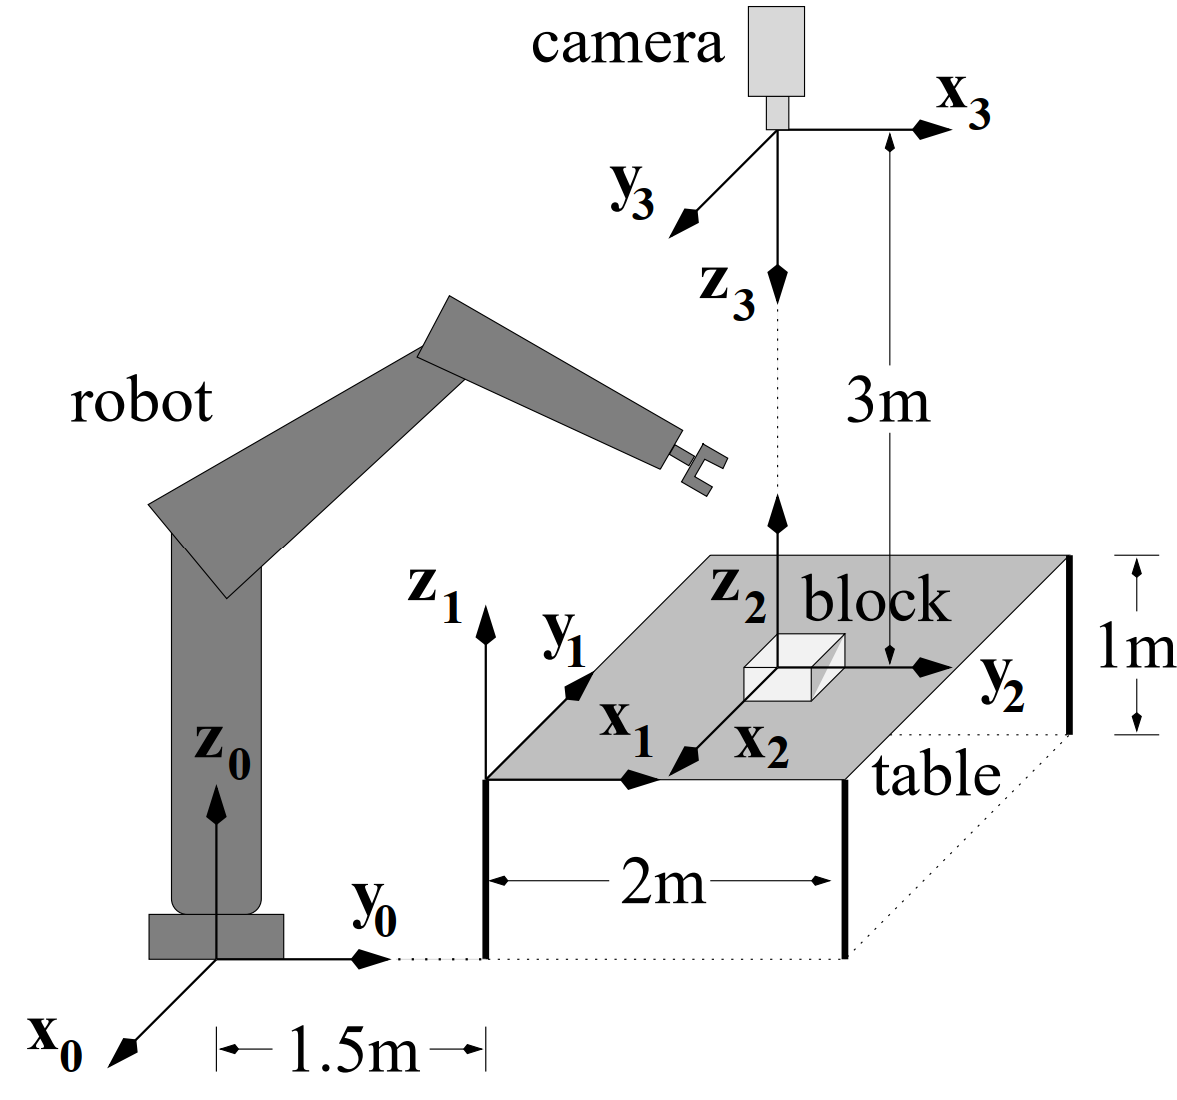
\includegraphics[width=.4\columnwidth]{figures/robot_arm_table_hollerbach.png}
	\centering
	\caption{}
	\label{fig:p5}
\end{figure}
\begin{enumerate}[label=(\alph*)]
    \item Find $\prescript{0}{}{\boldsymbol{T}}_{1}$, $\prescript{1}{}{\boldsymbol{T}}_{2}$, $\prescript{2}{}{\boldsymbol{T}}_{3}$, and $\prescript{0}{}{\boldsymbol{T}}_{3}$ by inspection.
    \item Assume the block has moved. It is tracked by the camera and is known
to exist at location $\prescript{3}{}{\boldsymbol{d}}_{32} = [-0.5 \quad 0.5 \quad 3]^{\intercal}$. Where is the block in the robot’s coordinate system, i.e., what is $\prescript{0}{}{\boldsymbol{d}}_{02}$?
\end{enumerate}

\end{problem}


\end{document}